%==============================================================================
% presentation.tex
%==============================================================================


%==============================================================================
% Configuration
%==============================================================================

% Internationalisation
\usepackage[utf8]{inputenc}
\usepackage[T1]{fontenc}
% \usepackage[ngerman]{babel}

% Different packages
\usepackage{url}
\usepackage{color,listings,paralist}
\usepackage{enumerate}
\usepackage{tabularx}

% Use default Acrobat reader fonts
\usepackage{mathpazo}

% Use CM fonts (increases document size)
\usepackage{ae}

% Use images
\usepackage{graphicx}

% Configure beamer
\usetheme[secheader]{Ikhono}
\usefonttheme[onlylarge]{structurebold}
\setbeamertemplate{navigation symbols}{}

% Variables
\providecommand{\Title}{Mining Software Repositories for Intelligent
  Software Maintenance}
\providecommand{\ShortTitle}{Mining software repositories}
\providecommand{\Author}{Thomas Weibel <weibelt@ethz.ch>}
\providecommand{\Institute}{SETLabs, Infosys Tech. Ltd., Bangalore}
\providecommand{\Date}{December 1, 2009}

% PDF settings
\hypersetup{
  pdftitle={\Title},
  pdfauthor={\Author},
  pdfsubject={\Institute},
  pdfkeywords={software engineering, portable, efficient, parallel
    programming language} 
}

% Titlepage
\title[\ShortTitle]{\Title}
\author{\Author}
\institute{\Institute}
\date{\Date}


%==============================================================================
% Document
%==============================================================================

\begin{document}


% Titlepage
\begin{frame}[plain]
  \titlepage
\end{frame}

\note{
  \begin{itemize}
  \item Hi and welcome to my presentation.
  \end{itemize}
}


\section*{Introduction}

\begin{frame}{Executive Summary}
  \begin{itemize}
  \item TODO
  \item Software repository mining for preventive maintenance
  \end{itemize}
\end{frame}

\note{
  \begin{itemize}
  \item TODO
  \end{itemize}
}


\section{Software Repository Mining}


\begin{frame}{Outline}
  \tableofcontents[current]
\end{frame}

\note{
  TODO
}

\begin{frame}{Version Control}
  \begin{center}
    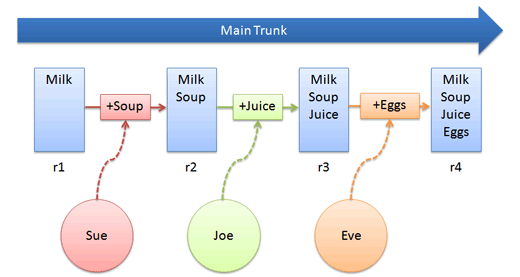
\includegraphics[scale=0.35]{figures/vcs}
  \end{center}

  \vspace{\stretch{1}}

  \begin{itemize}
  \item Management of changes to computer files in a repository
  \item Changes identified by a number or letter code (``revision'')
  \item Each revision associated with timestamp and person
    making the change
  \item Working copy: Local copy of files from a repository
  \end{itemize}
\end{frame}

\note{
  \begin{itemize}
  \item Version control is the management of changes to documents,
    programs, and other information stored as computer files. It is
    most commonly used in software development, where a team of people
    may be changing the same files.
  \item Changes are usually identified by a number or letter code,
    termed the ``revision''. For example, an initial set of files is
    ``revision 1''. When the first change is made, the resulting set
    is ``revision 2'', and so on.
  \item Each revision is associated with a timestamp and the person
    making the change.
  \item The working copy is the local copy of files from a repository,
    at a specific time or revision.
  \end{itemize}
}

\begin{frame}[fragile]{Commits and Change Sets}
  \begin{itemize}
  \item Commit: Writing changes to the working copy into the
    repository
  \item Change set: Set of changes made in a single commit
  \end{itemize}

  \vspace{\stretch{1}}

\begin{verbatim}
commit 3d2d827f5ca5e32816194119d5c980c7e04474a6
Author: Michael S. Tsirkin <mst@redhat.com>
Date:   Mon Sep 21 17:03:51 2009 -0700

    mm: move use_mm/unuse_mm from aio.c to mm/

M       fs/aio.c
A       include/linux/mmu_context.h
M       mm/Makefile
A       mm/mmu_context.c
\end{verbatim}
\end{frame}

\note{
  \begin{itemize}
  \item A commit occurs when a copy of the changes made to the working
    copy is written or merged into the repository.
  \item On version control systems with atomic multi-change commits, a
    change set identifies the set of changes made in a single commit.
  \end{itemize}
}

\begin{frame}{Software Repository Mining}
  TODO
\end{frame}

\note{
  TODO

  When mining software archives, we want to learn from the past to
  shape the future.

  All this contributes to the rise of a new field, the mining of
  software archives, which is concerned with the automated extraction,
  collection, and abstraction of information from available software
  development data. In past years, mining software archives has become
  one of the fastest-rising areas in software development
  research. Its promise is not only to provide insights into actual
  development processes but also to provide tools and techniques that
  let anyone gather such insights with as little collection and
  modeling effort as possible.
}

\begin{frame}{Frequent Item Set Mining}
  TODO
\end{frame}

\note{
  TODO
}


\section{Maintenance Challenges}

\begin{frame}{Outline}
  \tableofcontents[current]
\end{frame}

\note{
  TODO
}

\begin{frame}{Maintenance Challenges}
  TODO
\end{frame}

\note{
  TODO
}

\begin{frame}{Debugging}
  TODO
\end{frame}

\note{
  TODO
}

\begin{frame}{Impact Analysis}
  TODO
\end{frame}

\note{
  TODO
}

\begin{frame}{Predicting Faults}
  TODO
\end{frame}

\note{
  TODO
}

\begin{frame}{Predicting Changes}
  TODO
\end{frame}

\note{
  TODO
}

\begin{frame}{Code Ownership}
  TODO
\end{frame}

\note{
  TODO
}

\begin{frame}{Change Localization}
  TODO
\end{frame}

\note{
  TODO
}


\section{Framework}

\begin{frame}{Outline}
  \tableofcontents[current]
\end{frame}

\note{
  TODO
}

\begin{frame}{Architecture}
  \vspace{\stretch{1}}

  \begin{center}
    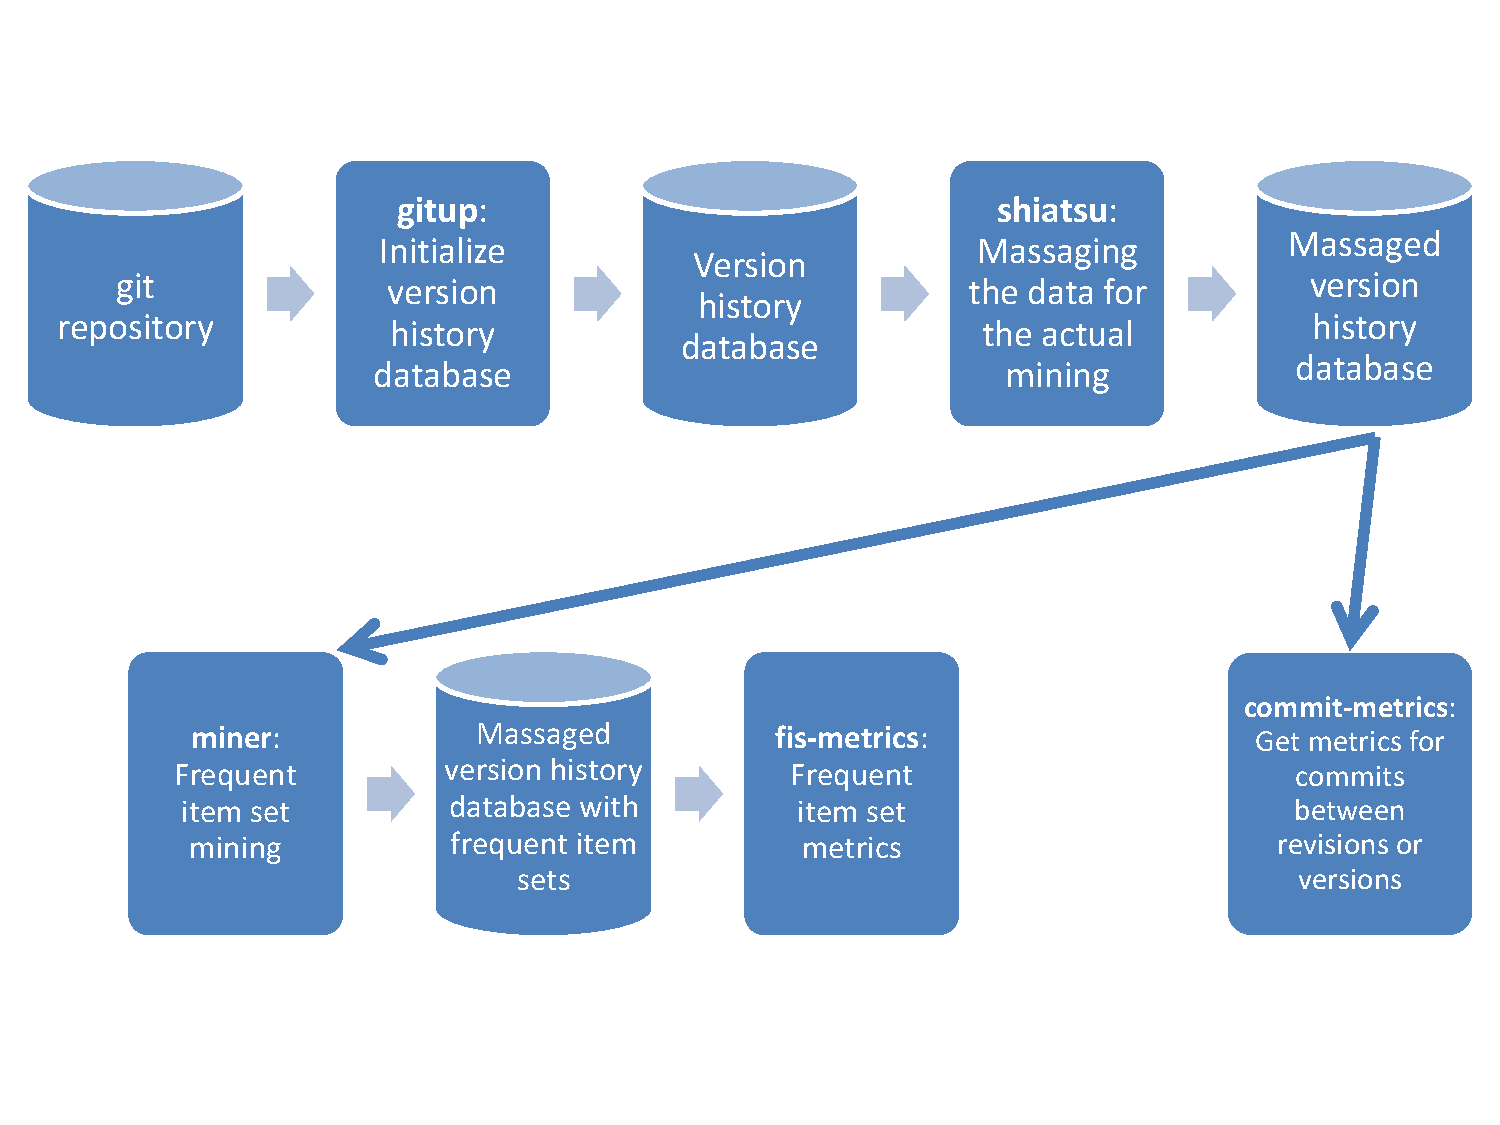
\includegraphics[width=\textwidth]{figures/miner-architecture}
  \end{center}

  \vspace{\stretch{1}}
\end{frame}

\note{
  TODO
}

\begin{frame}{Git}
  \begin{itemize}
  \item Free distributed version control system
  \item Initially designed and developed for Linux kernel development
  \item Every Git working directory is a full-fledged repository with
    complete history and full revision tracking capabilities, not
    dependent on network access or a central server.
  \item Repositories of other version control systems like CVS or
    Subversion can easily be converted into Git repositories
  \end{itemize}
\end{frame}

\note{
  \begin{itemize}
  \item Git is a free distributed version control system.
  \item Git was initially designed and developed by Linus Torvalds for
    Linux kernel development.
  \item Every Git working directory is a full-fledged repository with
    complete history and full revision tracking capabilities, not
    dependent on network access or a central server.
  \item Repositories of other version control systems like CVS or
    Subversion can easily be converted into Git repositories
  \end{itemize}
}


\section{Novelty}

\begin{frame}{Outline}
  \tableofcontents[current]
\end{frame}

\note{
  TODO
}

\begin{frame}{Change Localization Metrics}
  TODO
\end{frame}

\note{
  TODO
}

\begin{frame}{Experiments}
  \begin{itemize}
  \item Linux 2.6
    \begin{itemize}
    \item TODO
    \end{itemize}
  \item Wine
    \begin{itemize}
    \item TODO
    \end{itemize}
  \end{itemize}
\end{frame}

\note{
  TODO
}

\begin{frame}{Linux 2.6: Commit Metrics}
  \vspace{\stretch{1}}

  \begin{center}
    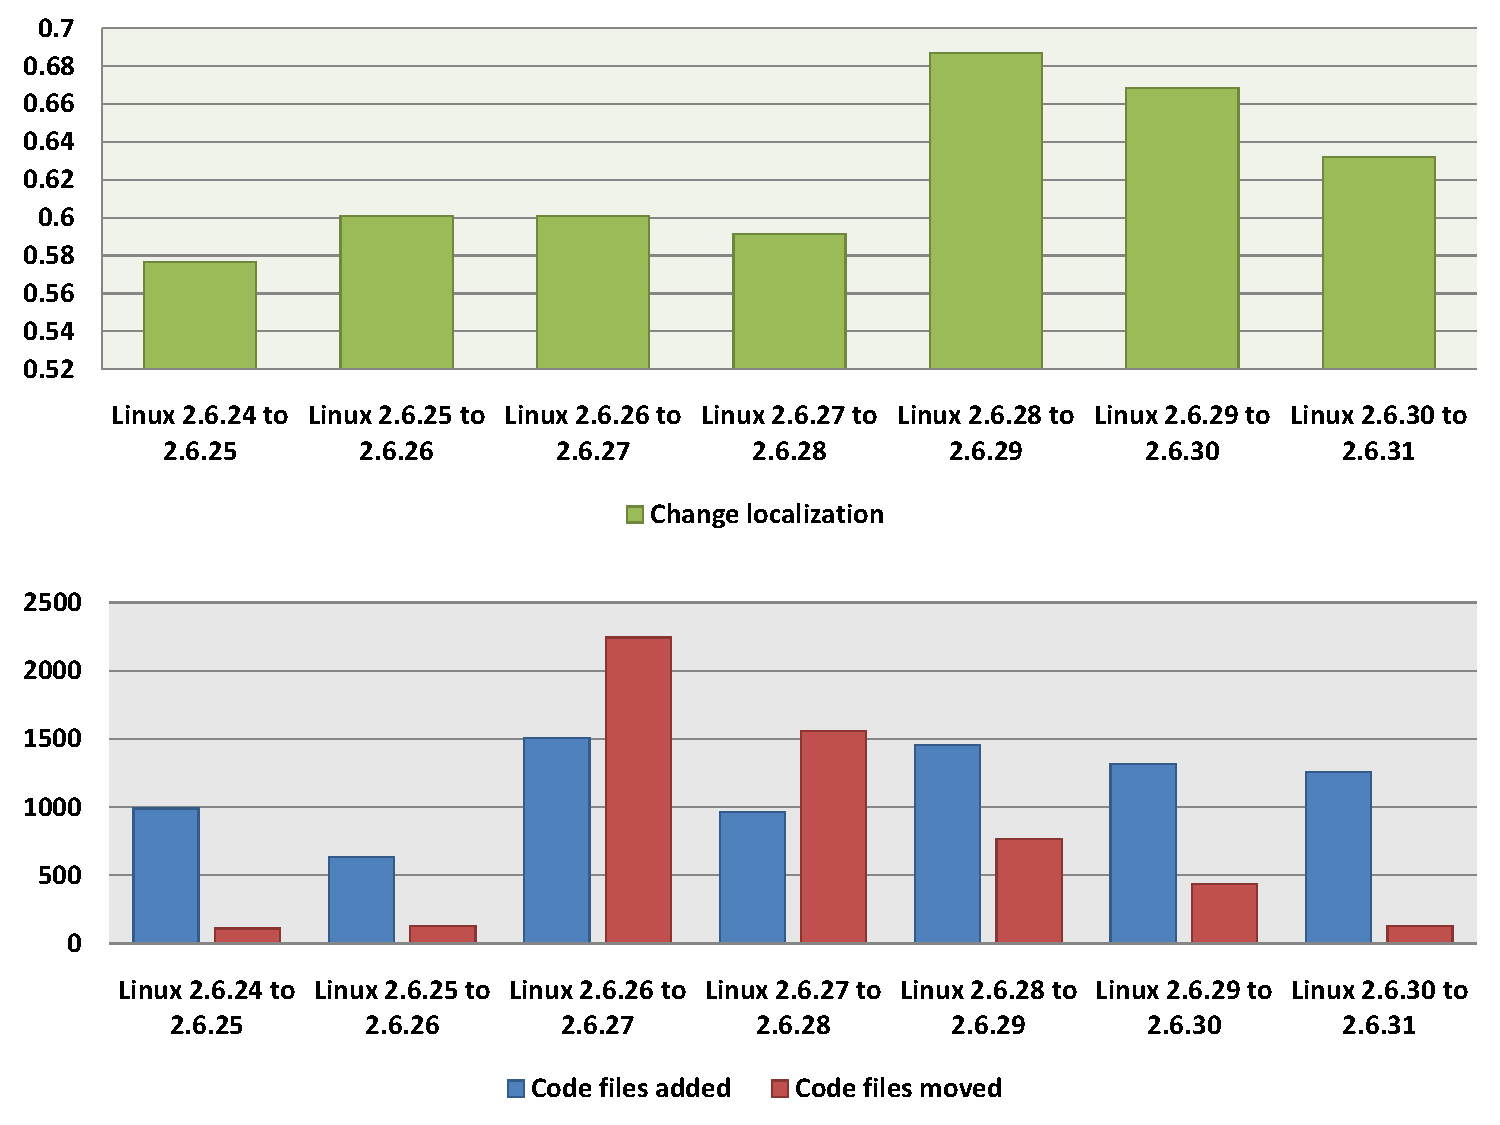
\includegraphics[width=0.95\textwidth]{minings/linux-2-6-commit-metrics}
  \end{center}

  \vspace{\stretch{1}}
\end{frame}

\note{
  TODO
}

\begin{frame}{Linux 2.6: Frequent Item Set Metrics}
  \vspace{\stretch{1}}

  \begin{center}
    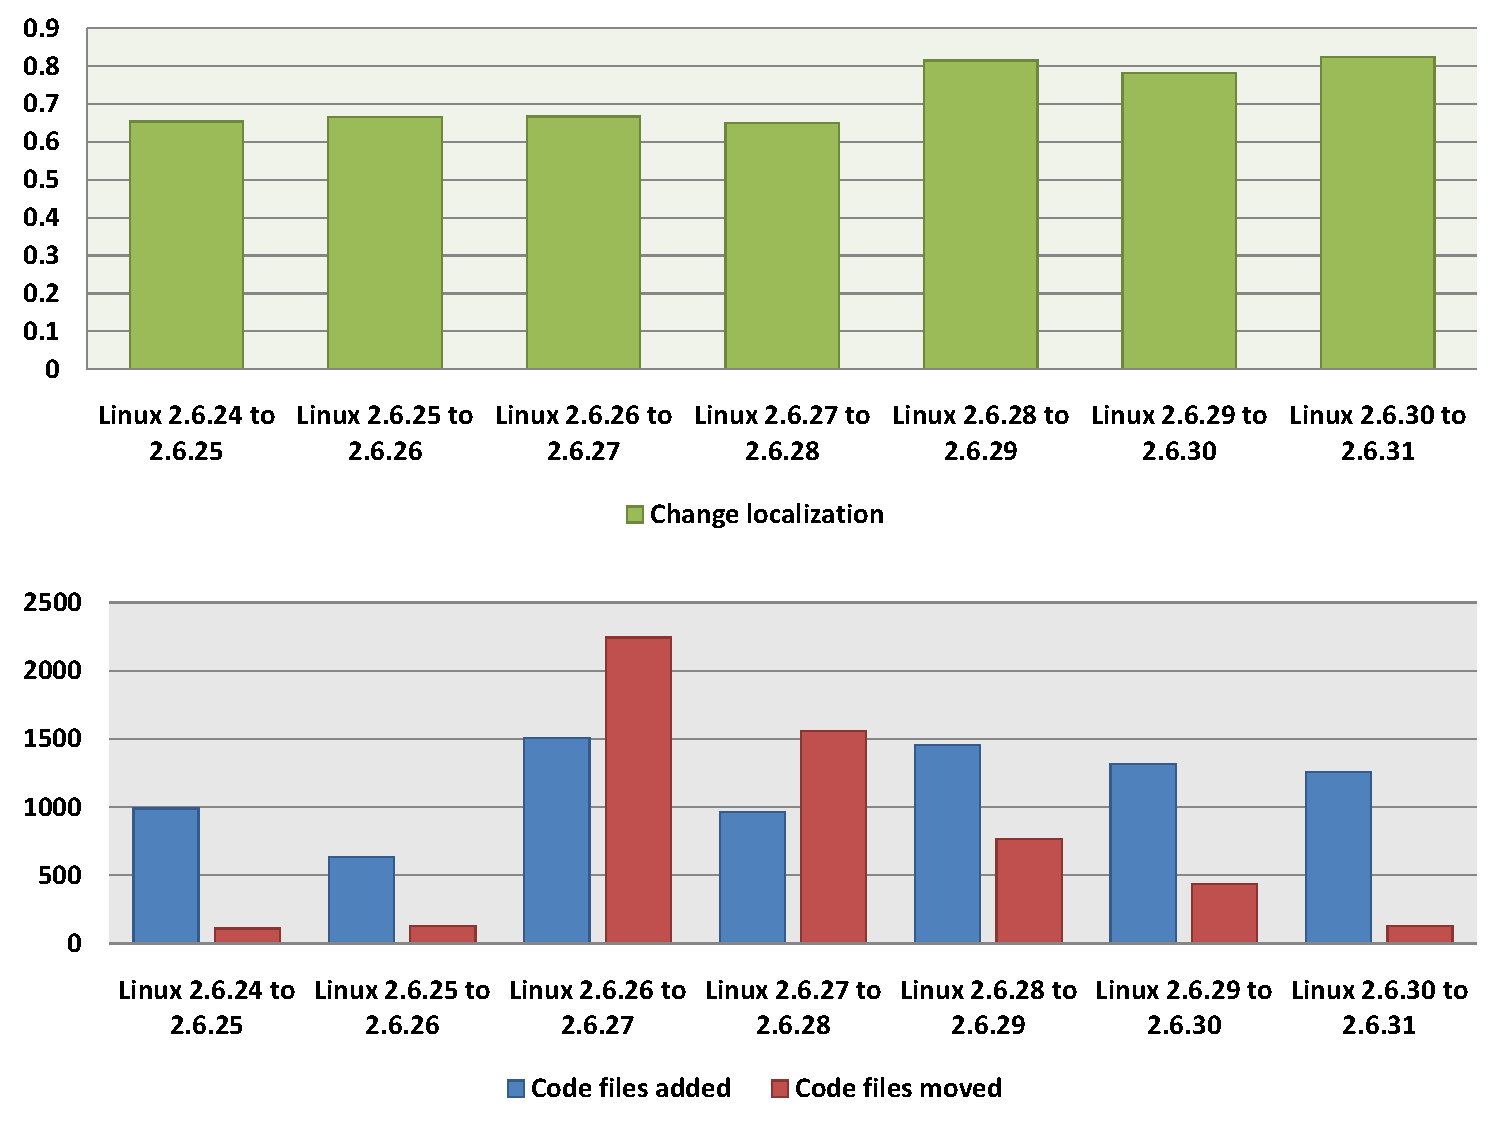
\includegraphics[width=0.95\textwidth]{minings/linux-2-6-fis-metrics}
  \end{center}

  \vspace{\stretch{1}}
\end{frame}

\note{
  TODO
}

\begin{frame}{Wine: Commit Metrics}
  \vspace{\stretch{1}}

  \begin{center}
    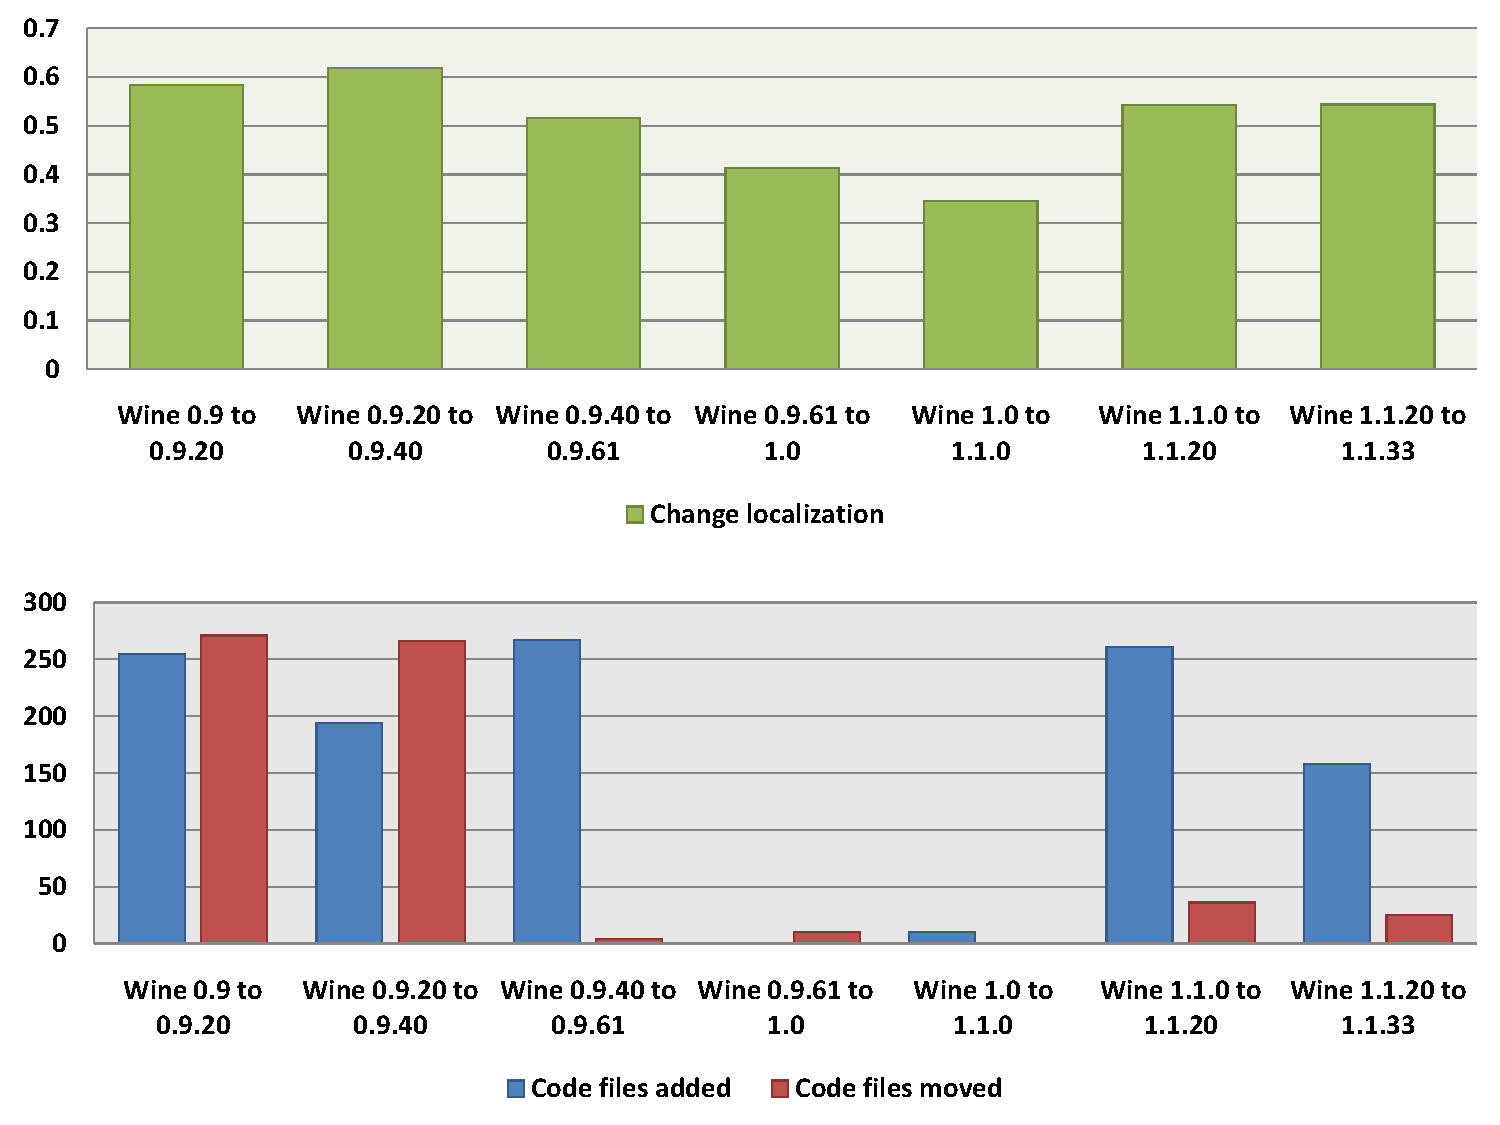
\includegraphics[width=0.95\textwidth]{minings/wine-commit-metrics}
  \end{center}

  \vspace{\stretch{1}}
\end{frame}

\note{
  TODO
}

\begin{frame}{Wine: Frequent Item Set Metrics}
  \vspace{\stretch{1}}

  \begin{center}
    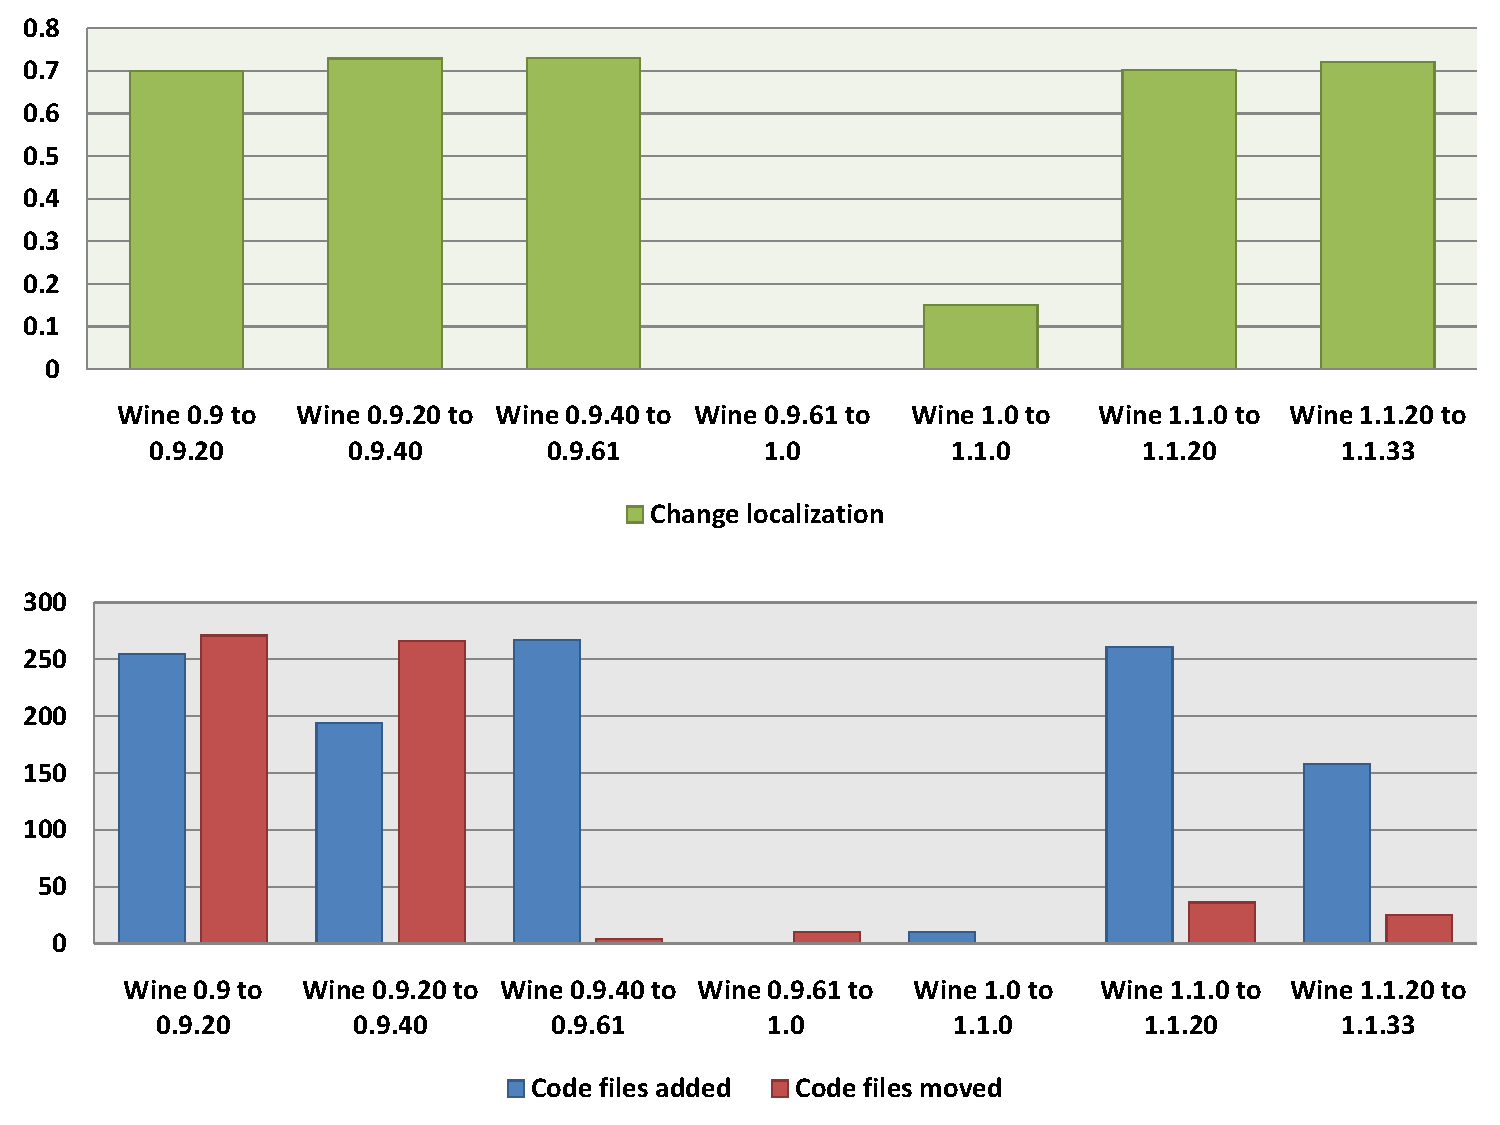
\includegraphics[width=0.95\textwidth]{minings/wine-fis-metrics}
  \end{center}

  \vspace{\stretch{1}}
\end{frame}

\note{
  TODO
}

\begin{frame}{Insights}
  \begin{itemize}
  \item TODO
  \item Moves increase localization
  \item Adds clear out moves
  \item Stable: mostly bugfixes -> low localization, only very few
    moves and adds
  \item Unstable: adding new features -> high localization, many moves
    and adds
  \end{itemize}
\end{frame}

\note{
  TODO
}


\section{Improving Software Maintainability}

\begin{frame}{Outline}
  \tableofcontents[current]
\end{frame}

\note{
  TODO
}

\begin{frame}{Maintenance Challenges}
  TODO
\end{frame}

\note{
  TODO
}

\begin{frame}{Debugging}
  TODO
\end{frame}

\note{
  TODO
}

\begin{frame}{Impact Analysis}
  TODO
\end{frame}

\note{
  TODO
}

\begin{frame}{Predicting Faults}
  TODO
\end{frame}

\note{
  TODO
}

\begin{frame}{Predicting Changes}
  TODO
\end{frame}

\note{
  TODO
}

\begin{frame}{Code Ownership}
  TODO
\end{frame}

\note{
  TODO
}

\begin{frame}{Change Localization}
  TODO
\end{frame}

\note{
  TODO
}


\section*{Outro}

\begin{frame}{Future Work}
  TODO
\end{frame}

\note{
  TODO
}

\begin{frame}{References}
  TODO
\end{frame}

\note{
  TODO
}

\begin{frame}{Conclusion}
  TODO
\end{frame}

\note{
  TODO
}

\end{document}
